\begin{table}[htpb]
    \centering
    \caption{Some short unfamiliar terminologies in Remaining chapter}
        \textit{The noting of Section 2-4 are skipped.}
    {\small
    \begin{tabular}{cp{32em}}
        \toprule
        Terminology & Explanations \\
        \midrule
        \textbf{BIC} & $\text{BIC}(K) = \log p(\mathcal{D}|\hat{\bm{\theta}}_k) - \frac{D_K}{2}\log N$, $D_K$ is the number of parameters in a model with $K$ clusters \\
        \textbf{label switching problem} & permuting the labels in a mixture model without changing the likelihood. \\
        \textbf{ordering constraint} & $\ell'(\bm{\theta}) = \log p(\mathcal{D}|\bm{\theta})+\log p(\bm{\theta})+\phi(\bm{\mu})$, 
        where $\phi(\bm{\mu})=-\infty$ if $\mu_1<\mu_0$ else $0$, where $\bm{\mu}$ is the label. \\
        \textbf{Collaborative filtering} & $\hat{Y}_{u,i}=\sum_{u':Y_{u',i}\neq ?}\mathrm{Sim}(u,u')Y_{u',i}$, 
        users collaborate on recommending items by sharing their ratings with other users \\
        \textbf{Matrix factorization} & $\mathcal{L}(\mathbf{Z}) = \|\mathbf{UV}^\mathsf{T}-\mathbf{Y}\|_\mathsf{F}^2$, $\mathbf{U}\in\mathbb{R}^{M\times K}$ and $\mathbf{V}\in\mathbb{R}^{N\times K}$, optimized by \textbf{ALS} or SGD when with missingness, and user-/item-specific baselines and penalty constraints can be added. \\
        \textbf{ALS} & Alternative least squares, estimating $\mathbf{U}$ given $V$ and vice versa \\
        \textbf{PMF} & Probabilistic matrix factorization, $p(y_{ui}=y)=\mathcal{N}(y|\mu+b_u+c_i+\bm{u}_u^\mathsf{T}\bm{v}_i,\sigma^2)$, allowing discrete distribution and regarding r/c symmetrically. \\
        \textbf{AutoRec} & $f(\bm{y}_{\cdot,i};\bm{\theta})=\mathbf{W}^\mathsf{T}\varphi(\mathbf{V}\bm{y}_{\cdot,i}+\bm{\mu})+\bm{b}$,
        \textit{item-based} nonlinear version of MF, there is also \textit{user-based}.\\
        \textbf{BPR} loss & Bayesian personalized ranking loss, $\mathcal{L}(\bm{\theta})=\sum_{(u,i,j)\in\mathcal{D}}\log \sigma(f(u,i;\bm{\theta})-f(u,j;\bm{\theta}))-\lambda\underbrace{\|\bm{\theta}\|^2}_{\mathcal{N}~\text{prior}}$, where $\mathcal{D}=\left\{(u,i,j):i\in\mathcal{I}_u^+,j\in\mathcal{I}\setminus\mathcal{I}_u^+\right\}$
        \textit{still asymmetrically}\\
        % \textbf{FM} & Factorization machines,  \\
        \textbf{GDL} & Geometric Deep Learning, applying deep learning techniques to non-Euclidean data \\
        \textbf{GRL} & Graph Representation Learning, learning low-dimensional continuous vector representations for graph-structured data, also called embedding \\
        \textbf{transductive} & the graph structure can be fixed throughout training and testing \\
        \textbf{inductive} & expecting to inference the info of graphs not seen during training \\
        \textbf{shallow graph embeddings} & $\mathbf{Z}=\mathrm{ENC}(\mathbf{\Theta}^E)\triangleq \mathbf{\Theta}^E$ where $\mathbf{\Theta}^E\in\mathbb{R}^{N\times L}$, the embedding dictionary $\mathbf{Z}$ is directly learned as model parameters, \textit{recall PCA} \\
        % \textbf{DeepWalk} & $\mathcal{L}_{G,\text{rec}}(\mathbf{W},\hat{\mathbf{W}};\mathbf{\Theta})=\log$ \\
        \textbf{Label propagation} & $\mathcal{L}_{G,\text{rec}}(\mathbf{W},\hat{\mathbf{W}};\mathbf{\Theta})=\sum_{i,j}W_{i,j}\|\bm{y}_i^N-\hat{y}_j^N\|^2_2$ \\
        \textbf{Label spreading} & $\mathcal{L}_{G,\text{rec}}(\mathbf{W},\hat{\mathbf{W}};\mathbf{\Theta})=\sum_{i,j}W_{i,j}\left\|\frac{\bm{y}_i^N}{\sqrt{D_i}}-\frac{\hat{y}_j^N}{\sqrt{D_j}}\right\|^2_2$ \\
        \bottomrule
    \end{tabular}}
    \label{tab:rest}
\end{table}




\subsection{Clustering}

Evaluating the clustering: to assign points that are similar to the same cluster, 
and to ensure that points that are dissimilar are in different clusters:
\begin{itemize}
    \item \textbf{Purity}: let $N_{ij}$ be the number of objects in cluster $i$ that belong to class $j$
    \begin{gather}
        \text{purity} \triangleq \sum_i
        \underbrace{\frac{\cancel{N_{i\cdot}}}{N_{\cdot\cdot}}}_\text{\makecell{cluster\\weight}}
        \underbrace{\max_j\frac{N_{ij}}{\cancel{N_{i\cdot}}}}_\text{\makecell{cluster\\purity}}
    \end{gather}

    \item \textbf{Rand index}: let $U=\{u_1,\cdots,u_R\}$ (estimated clustering) and 
    $V=\{v_1,\cdots,v_C\}$ (reference clustering) be two different \textit{partitions} of $N$ data points,
    and consider pairs of data points $(x_i,x_j)$\unsure{Hint: there are $\binom{N}{2}$ pairs.}
    having following relationship annotated by the two clustering labels:
    \begin{center}
        \begin{tabular}{ccc}
            \toprule
            estimated labels & reference labels & Notation \\
            \midrule
            $y^U_i = y^U_j$ & $y^V_i=y^V_j$ & $\mathrm{TP}$ \\
            $y^U_i \neq y^U_j$ & $y^V_i \neq y^V_j$ & $\mathrm{TN}$ \\
            $y^U_i \neq y^U_j$ & $y^V_i = y^V_j$ & $\mathrm{FN}$ \\
            $y^U_i = y^U_j$ & $y^V_i \neq y^V_j$ & $\mathrm{FP}$ \\
            \bottomrule
        \end{tabular}
    \end{center}
    \begin{gather}
        R \triangleq \frac{\mathrm{TP} + \mathrm{TN}}{\mathrm{TP} + \mathrm{FP} + \mathrm{FN} + \mathrm{TN}} \\
        R_\text{adj} \triangleq \frac{R-\mathbb{E}R}{\max R - \mathbb{E}R},
    \end{gather}
    where the randomness is based on using the \textit{generalized hyper-geometric distribution}.

    \item \textbf{Mutual information}: same notation as the above
    \begin{gather}
        p_{UV}(i,j)=\frac{|u_i\cap v_j|}{N},~p_U(i)=\frac{|u_i|}{N},~p_V(j)=\frac{|v_j|}{N} \\
        \mathbb{I}(U,V) = \sum_{i=1}^R\sum_{j=1}^C p_{UV}(i,j)\log\frac{p_{UV}(i,j)}{p_U(i)p_V(j)} \\
        \mathbb{I}_\text{norm} \triangleq \frac{\mathbb{I}(U,V)}{(\mathbb{H}(U) + \mathbb{H}(V))/ 2}
    \end{gather}
\end{itemize}

\textbf{Hierarchical agglomerative clustering} (HAC): from disimilarity matrix $\mathbf{D}\in \mathbb{R}^{N\times N}$ 
$\to$ a \textit{tree structure} in which the most similar pair are grouped together \textit{in a hierarchical fashion},
the update strategies include
\begin{itemize}
    \item \textbf{Single link}, \textit{nearest neighbor clustering} ($O(N^2)$): $d_{SL}(G,H)=\min_{i\in G,i'\in H}d_{i,i'}$
    \item \textbf{Complete link}, \textit{further neighbor clustering} ($O(N^3)$): $d_{CL}(G,H)=\max_{i\in G,i'\in H}d_{i,i'}$
    \item \textbf{Average link} ($O(N^3)$): $d_{avg}(G,H)=\frac{1}{n_Gn_H}\sum_{i\in G,i'\in H}d_{i,i'}$
\end{itemize}

\textbf{K means clustering} updates $K$ cluster centers\unsure{It is sensitive to the initial values for $\bm{\mu}_k$,
thus a robust result requires multiple initiations in practice.} 
in each iteration according to current clustering result, 
which runs in $O(NKT)$ time.\unsure{same with \textbf{vector quantization}, a approach of lossy compression of real-valued vectors: $\bm{x}_n\in \mathbb{R}^D\to z_n\in\{1,\cdots,K\}$}
\begin{align}
    & \begin{cases}
        z_n^* = \argmin_k{\color{red}\|\bm{x}_n-\bm{\mu}_k\|_2^2} \\
        \bm{\mu}_k={\color{blue}\frac{1}{N_k}\sum_{n:z_n=k}\bm{x}_n}
    \end{cases} \\
    \iff \min~&~J(\mathbf{M},\mathbf{Z}) \\
    \mathrm{s.t.}~&~J(\mathbf{M},\mathbf{Z}) = \sum_{n=1}^N\|\bm{x}_n-\bm{\mu}_{z_n}\|^2=\|\mathbf{X}-\underbrace{\mathbf{ZM}^\mathsf{T}}_{\text{enc-dec}}\|^2_\mathsf{F} \\
    & \mathbf{X}\in\mathbb{R}^{N\times D},~\mathbf{Z}\in [0,1]^{N\times K},~\mathbf{M}\in\mathbb{R}^{D\times K}
\end{align}
\begin{itemize}
    \item \textbf{K-means++}: choosing the center points sequentially and with probability increasing with the distance to the nearest existing centroids,
    i.e. \textit{the points far away from a centroid are more likely to be picked}.
    \begin{gather}
        P(\bm{\mu}_t=\bm{x}_n) = \frac{D_{t-1}(\bm{x}_n)}{\sum_{n'=1}^ND_{t-1}(\bm{x}_{n'})} \\
        D_t(\bm{x}) = \min_{1\leq k \leq t-1} \|\bm{x}-\bm{\mu}_k\|^2_2
    \end{gather}

    \item \textbf{K-medoids}: $m_{1:K}\in\{1,\cdots,N\}$\unsure{
    there are two differences between K-means and K-Medoids:
    \textcolor{red}{(1) the centroids of clusters in K-medoid are \textit{existing examples} 
    instead of the \textit{imagined center} of the data points in a cluster in K-means;}
    \textcolor{blue}{(2) distance in K-means is extended to dissimilarity in K-medoid}, 
    i.e. extending assumption of MMG to any mixture distributions, and K-means is a \textit{special case of EM}.
    Both can eliminate the effect of outliers.
    }
    \begin{gather}
        \text{repeat}~
        \begin{cases}
            z_n=\argmin_k {\color{red}d(\bm{x}_n,\bm{x}_{m_k})} \\
            m_k={\color{blue}\argmin_{n:z_n=k} \sum_{n':z_{n'}=k} d(x_n,x_{n'})}
        \end{cases}~\text{for}~k=1:K    
    \end{gather}
\end{itemize}

\textbf{Silhouette coefficient} $\to$ silhouette score $\to$ silhouette diagram
\begin{gather}
    \mathrm{SC}(i) = \frac{(b_i-a_i)}{\max(a_i,b_i)},
\end{gather}
where $a_i$ is the mean distance to the other instances in cluster $k_i$, measuring the \textit{compactness} of $i$'s cluster,
and $b_i$ is the mean distance to the other instance in the next \textit{closest} cluster $k'_i$, measuring the \textit{distance} between the clusters.

\textbf{Spectral clustering} uses the \textit{eigenvectors} to derive \textit{feature vectors} for each datapoint 
and then cluster them by feature-based clustering methods.\unsure{
Considering the similarity matrix is inefficient in storage if $N>D$ or the recovering is irreversible if $N<D$,
why is the similarity matrix needed?}
Let $\mathbf{U}\in\mathbb{R}^{N\times K}$ be the $K$ eigenvectors of $\mathbf{L}$\unsure{
Usually, the graph Laplacian should be normalized to account for the nodes with significant centrality.
$\mathbf{L}_\text{sym}\triangleq\mathbf{L}^{-\frac{1}{2}}\mathbf{LD}^{-\frac{1}{2}}$
} with the \textit{smallest eigenvalues} in its columns\unsure{``bottom'' eigenvectors}
and $\bm{u}_i\in\mathbb{R}^K$ be the $i$th \textit{row} of $\mathbf{U}$.
Then by Theorem \ref{thm:lapblock}, these $\bm{u}_i$ will be piecewise constant within connected components under ideal condition,
then we can apply regular clustering methods to $\mathbf{U}$ to recover the connected components.
It is closely related to \textbf{kPCA} (using largest eigenvectors of $\mathbf{W}$ is equivalent to the smallest ones of $\mathbf{I}-\mathbf{W}$) and 
\textbf{random walk analysis} ($\mathbf{P}=\mathbf{D}^{-1}\mathbf{W}=\mathbf{I}-{\mathbf{L}_\text{rw}}_{\color{gray}\triangleq \mathbf{D}^{-1}\mathbf{L}}$
is a stochastic matrix, interpreted as the probability of going from $i$ to $j$.)

\begin{theorem}\label{thm:lapblock}
    Consider the graph Laplacian, $\mathbf{L}\triangleq \mathbf{D}-\mathbf{W}$,
    where $\mathbf{W}$ is a symmetric weight matrix for the graph, $\mathbf{D}=\mathrm{diag}(d_i)$, and $d_i=\sum_j w_{ij}$.
    
    The $\mathbf{L}$'s eigenvectors with eigenvalue 0 is spanned by the indicators vectors 
    $\mathbf{1}_{|\mathcal{S}_k|}$,
    $k=1,\cdots,K$, where $\mathcal{S}_k$'s are the $K$ groups of connected nodes of the graph.
\end{theorem}
\begin{proof} $~$
    \begin{itemize}[Case]
        \item $K=1$\\
        Let $\bm{f}$ is an eigenvector with eigenvalue 0, then $0=\sum_{ij}w_{ij}(f_i-f_j)^2$, since
        \begin{align}
            0 
            & = \bm{f}^\mathsf{T}\mathbf{L}\bm{f} = \bm{f}^\mathsf{T}(\mathbf{D}-\mathbf{W})\bm{f}\\
            & = \bm{f}^\mathsf{T}\begin{bmatrix}
            \sum_j w_{1j} & -w_{12} & \cdots & -w_{1N} \\
            -w_{21} & \sum_j w_{2j} & \cdots & -w_{2N} \\
            \vdots & \vdots & \ddots & \vdots \\
            -w_{N1} & -w_{N2} & \cdots & \sum_j w_{Nj}
            \end{bmatrix}\bm{f} \\
            & = \sum_{k}f_k\left(f_k\sum_jw_{kj}-\sum_if_iw_{ik}\right)~~{\color{gray}(w_{ii}=0)} \\
            & = \sum_{ij}f_i(f_i-f_j)w_{ij} \\
            & = \underbrace{\sum_{ij}f_i(f_i-f_j)w_{ij}}_{0} - \underbrace{\sum_{ij}f_j(f_i-f_j)w_{ij}}_{0} \\
            & = \sum_{ij}(f_i-f_j)^2w_{ij}
            % & = \sum_i f_i^2\sum_j w_{ij} - \sum_{ij} f_i f_j w_{ij} \\
            % & = \sum_i f_i \sum_j(f_i-f_j)w_{ij} \\
            % & = \sum_j f_j \sum_i(f_i-f_j)w_{ij} \\
            % & {\color{red}\overset{?}{=}\sum_{ij}(f_i-f_j)^2w_{ij}}
        \end{align}
        For any two connected nodes $i,j$, we have $w_{ij}>0$, then we must have that $f_i=f_j$ by the above result.
        Hence $\bm{f}$ is constant for all nodes connected by a path.

        \item $K>1$\\
        Then, $\mathbf{L}$ will be block diagonal. Then A similar argument to the above shows that we will have $K$ indicator functions.
    \end{itemize}
\end{proof}

\begin{figure}[htpb]
    \centering
    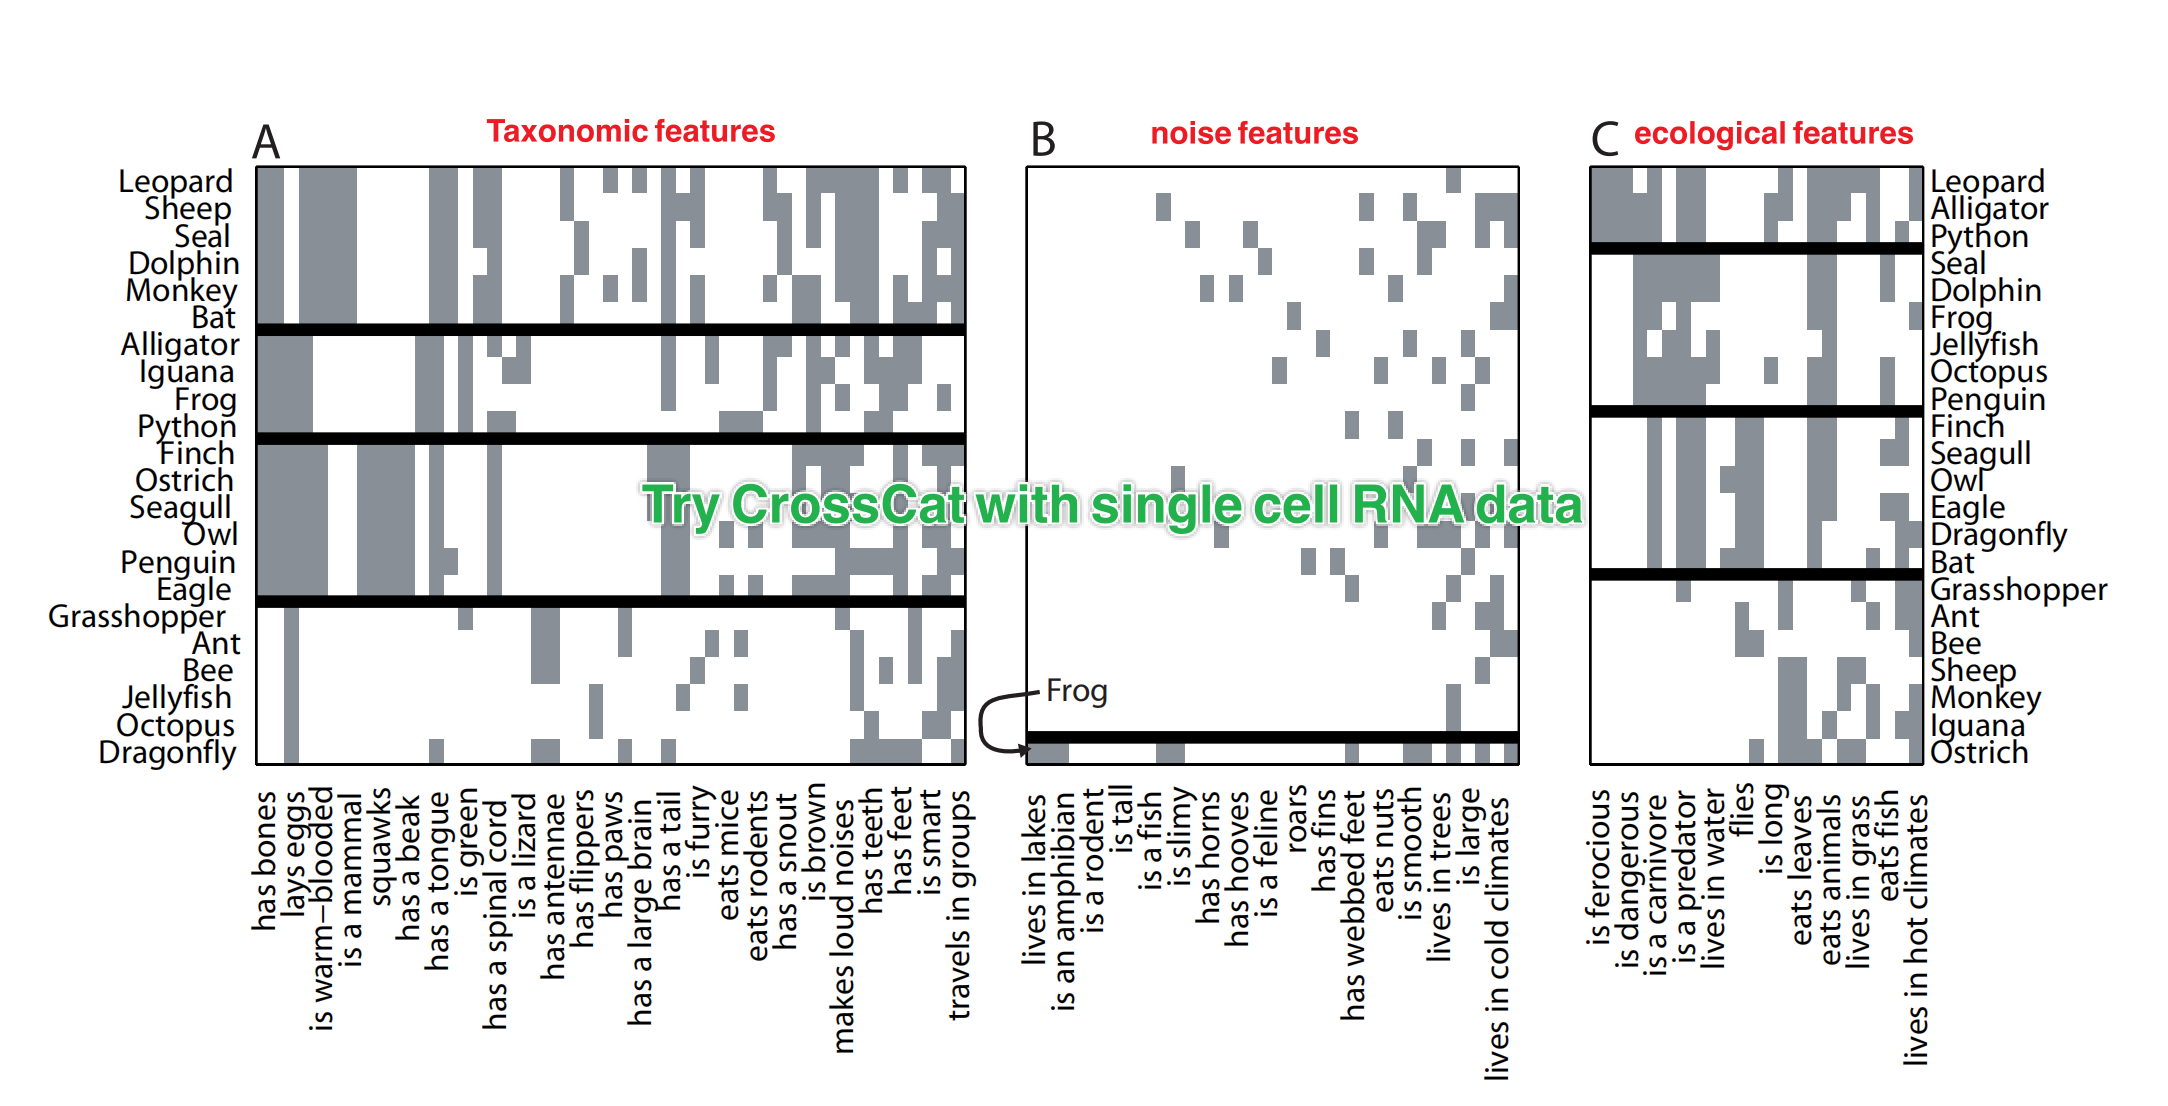
\includegraphics[width=\textwidth]{figs/crosscat.png}
    \caption{MAP estimate produced by the \textbf{CrossCat} system, \textbf{CrossCat}, nested partition models for biclustering.}
    \textit{It can be applied to scRNA data to discovery novel bi-label cell types}
    \label{fig:crosscat}
\end{figure}

\subsection{Graph Embeddings}

\begin{figure}[htpb]
    \centering
    \begin{tikzpicture}[
        datanode/.style={rectangle, solid, draw=black!85, rounded corners=.1cm, fill=orange!15, minimum size=10mm},
        networknode/.style={rectangle, solid, draw=black!85, rounded corners=.1cm, fill=violet!15, minimum size=10mm},
        lossnode/.style={rectangle, solid, draw=black!85, minimum size=10mm},
        dashedouter/.style={rectangle, draw=black!50, dashed, very thick, inner sep=5pt, inner xsep=2mm, inner ysep=3mm},
        dottedouter/.style={rectangle, draw=black!50, dotted, very thick, rounded corners=.2cm},
        ->,>=stealth',auto,node distance=7mm,thick]
        \tikzstyle{every node}=[font=\small,scale=0.9]

        \node[networknode] (enc) {$\mathrm{ENC}(\mathbf{W},\mathbf{X};\mathbf{\Theta}^E)$};

        % \node[dashedouter, label=above:{Input}] (input) {
        % \begin{tikzpicture}[remember picture]
            \node[datanode, left = of enc] (X) {$\mathbf{X}$};
            \node[datanode, below = of X] (W) {$\mathbf{W}$};
        % \end{tikzpicture}
        % };

        \node[fit={(X) (W)}, dashedouter, label=above:{Input}, inner xsep=2mm, inner ysep=3mm] (output) {};
        
        \node[datanode, right = of enc] (Z) {$\mathbf{Z}$};
        \node[networknode, right = of Z] (decs) {$\mathrm{DEC}(\mathbf{Z};\mathbf{\Theta}^S)$};
        \node[networknode, below = of decs] (decd) {$\mathrm{DEC}(\mathbf{Z};\mathbf{\Theta}^D)$};

        % \node[dashedouter, label=above:{Output}] (output) {
        % \begin{tikzpicture}[remember picture]
            \node[datanode, right = of decs] (haty) {$\hat{\bm{y}}^S$};
            \node[datanode, below = of haty] (hatW) {$\hat{\mathbf{W}}$};
        % \end{tikzpicture}
        % };
        
        \node[fit={(haty) (hatW)}, dashedouter, label=above:{Output}] (output) {};
        
        \node[lossnode, right = of haty] (ls) {$\mathcal{L}_\text{sup}^S$};
        \node[lossnode, below = of ls] (lr) {$\mathcal{L}_\text{rec}^G$};

        \node[datanode, right = of ls] (ys) {$\bm{y}^S$};
        % \node[datanode, right = of lr] (hatW) {$\mathbf{W}$};

        \node[fit={(X) (W) (enc) (Z)}, dottedouter, draw=NavyBlue!40, inner xsep=6mm, inner ysep=4mm, ultra thick] (graphencnet) {};
        \node[anchor=south] at ([yshift=0.1cm]graphencnet.north) {\color{NavyBlue}\makecell{\textbf{Graph encoder network}: \\ graph structure + optional node features \\ $\to$ node embeddings}};

        \node[fit={(W) (decd) (hatW) (lr)}, dottedouter, draw=ForestGreen!40, inner xsep=11mm, inner ysep=4mm, ultra thick] (graphdecdnet) {};
        \node[anchor=north] at ([yshift=-0.1cm]graphdecdnet.south) {\color{ForestGreen}\makecell{\textbf{Graph decoder network}: \\ node embeddings $\to$ similarity scores}};

        \node[fit={(Z) (decs) (haty) (ls) (ys)}, dottedouter, draw=Maroon!40, inner xsep=8mm, inner ysep=3mm, ultra thick] (graphdecsnet) {};
        \node[anchor=south] at ([yshift=0.2cm]graphdecsnet.north) {\color{Maroon}\makecell{\textbf{Classification network}: \\ node embeddings $\to$ labels}};

        \node[fit={(Z)}, dottedouter, draw=ForestGreen!40, inner xsep=5mm, inner ysep=5mm, ultra thick] (graphdecdnet1) {};
        
        \draw[->] (X) -- (enc);
        \draw[->] (W) -| (enc);
        \draw[->] (enc) -- (Z);
        \draw[->] (Z) -- (decs);
        \draw[->] (Z) |- (decd);
        \draw[->] (decs) -- (haty);
        \draw[->] (decd) -- (hatW);
        \draw[->, dashed] (haty) -- (ls);
        \draw[->, dashed] (hatW) -- (lr);
        \draw[<-] (ls) -- (ys);
        \draw[->, dashed] (W) |- +(0,-1)-| (lr);
        % \draw[<-, dashed] (hatW) -- (W);
    \end{tikzpicture}
    \begin{gather}
        \mathcal{L} = \alpha \mathcal{L}^S_\text{sup}(\bm{y}^S,\hat{\bm{y}}^S;\mathbf{\Theta})
        + \beta \mathcal{L}_{\text{rec}}^G(\mathbf{W},\hat{\mathbf{W}};\mathbf{\Theta})
        + \gamma \mathcal{L}_\text{reg}(\mathbf{\Theta})
    \end{gather}
    where $S\in\{N,E,G\}$, $\mathbf{\Theta}=\{\mathbf{\Theta}^N,\mathbf{\Theta}^E,\mathbf{\Theta}^G,\mathbf{\Theta}^D\}$ and $\mathcal{L}_\text{reg}$ is regularization term.
    The overall loss is composed of supervised losses (optional), reconstruction loss, and regularization loss with weights.
    \caption{Framework of \textsc{GraphEDM}}
    \label{fig:graphedm}
\end{figure}


\begin{center}
    \textit{
    The remaining contents are organized like review without enough details.
    }
\end{center}








